\documentclass[a4paper]{article}
\usepackage{graphicx}
\usepackage{float}

\input{style/head.tex}

%-------------------------------
%	TITLE VARIABLES (identify your work!)
%-------------------------------
%-------------------------------
%	TITLE VARIABLES (identify your work!)
%-------------------------------

\newcommand{\yourname}{Philippe BAZET} % replace YOURNAME with your name
\newcommand{\youremail}{pbazet@yahoo.com} % replace YOUREMAIL with your email
\newcommand{\assignmentnumber}{1} % replace X with the lab session number

\begin{document}

%-------------------------------
%	TITLE SECTION (do not modify unless you really need to)
%-------------------------------
\input{style/header.tex}

%-------------------------------
%	ASSIGNMENT CONTENT (add your responses)
%-------------------------------

\section{Question 1}

\subsection{Role of square mask}

Transformer model contains a self attention layer for computing attention vector of each token from input sentence. In \citep{Vaswani2017} the global self attention mechanism is modeled by following matrix formula assigning an attention vector to each input token in parallel

\begin{equation}
Attention(Q,K,V) = softmax(\frac{QK^{T}}{\sqrt(d_{k}})V
\end{equation}

For the self attention mechanism, each input token is compared to all other tokens in the input sentence and an attention vector is built which is a weighted sum of these comparaions. More formally, for a given input token, $Q$ matrix linearly project input token into a $q$ vector. Using dot product, the $q$ vector is compared to a $k_{i}$ vector assigned to all other $i$ token. $softmax$ function assign a weight to each comparaison between input token and all other input tokens.

The square mask removes from this comparaison mechanism between tokens, the tokens which are to the right of a given token. The language modeling task is an auto regressive task that learn tokens that are to the right of a given token. Thus, these right tokens should be removed from the input of the transformer. This operation is performed by assigning $-\infty$ value in matrix multiplication to vectors associated to these right tokens. Using softmax formula and usage of $exp$, these negative value will assign a zero weight for the tokens to the right of a given token.

\subsection{Role of positional encoding}

One big advantage of transformer model is to process simultaneously all tokens of an input sentence. This is a big improvement compared to recurrent neural network where each input tokens had to be processed sequentially. This parallel process requires to model position of token inside input sentence. This is achived by positional encoding.\\
To each embedding assigned to a token, positional embedding adds a vector of the same dimension modeling the position of token inside inout sentence. Assuming dimension of embedding for input token is $d_{model}$, for a given $position$, the positional encoding is modeled by vector $(PE_{(position,j)})$  where $j \in [0,d_{model}[$

\begin{equation}
PE_{(position,2i)}=sin(pos/1000^{2i/d_{model}})
\end{equation}

\begin{equation}
PE_{(position,2i+1)}=cos(pos/1000^{2i/d_{model}})
\end{equation}

\begin{figure}[H]
\centering
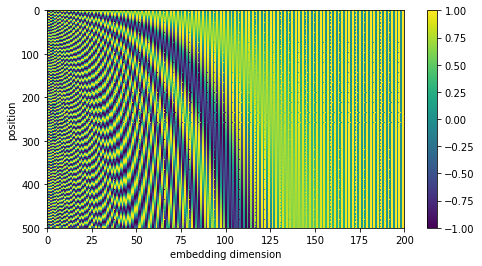
\includegraphics[scale=1.0]{figures/pos encoding.png}
\end{figure}

Objective of positional embedding is to add a bias between -1 and 1 to each dimension of embedding. Positional embedding is building such a way that combination of these biases accross dimensions of embedding are different from one position to the other positions.


\section{Question 2}

Objective of two tasks are diffrent and output dimensions are also different:
\begin{itemize}
\item \textit{Language modeling} task is a regression task that build a target sentence from a given input sentence. Input and output sentence are modeled by a list of integer. Each integer being an index into a vocabulary shared by input and output sentence
\item \textit{Classification} task learns a scalar from an input sentence. The scalar indexes list of finite elements for classifications to be learnt.
\end{itemize}
Both tasks use same output senetnce of embedding from transformer model. From this ouput, they build an other output sentence from integer. Usage of output sentence from classification head is different
\begin{itemize}
\item Language modeling builds an other sentence of same vocabulary as input sentence.
\item Classificatio task assigns to each element of output sentence a class by modeling each element by an integer being an index for the items of the classification to be learned. It assumes by traversing the output sentence accumulated evidences of the targeted class. It considers that class assigned to last element of ouput sentence is targeted class
\end{itemize}

\section{Question 3}

Given $d_{model}$ size of hidden embedding for tokens of input sentence, $\overline{V}$ size of vocabulary used for input tokens and $N$ number of targeted classes for \textit{classification} task,  \textit{language modeling} and \textit{classification} task share some common layers with same trainable parameters 
\begin{itemize}
\item Transformer Block. Associated parametrization will be detailed in following section
\item Positional Encoding Layer. This layer does not use any trainable parameters. Paramters are computed before training and are fixed. 
\item Embedding Layer. Dimension is $\overline{V} \times d_{model}$ parameter weights with $d_{model}$ biases
\end{itemize}

Additionnaly \textit{language modeling} and \textit{classification} use same component architecture for last layer: a linear layer followed by a softmax non linearity. Nonetheless, each task use different parametrization
\begin{itemize}
\item \textit{Language modeling} task converts the output of the Transformer Block into sentence of vectors having same dimension as vocabulary size $\overline{V}$. Number of trainable parameters is $\overline{V} \times d_{model}$ weights with additional $\overline{V}$ biases 
\item \textit{Classification} task converts the output of the transformer block into  sequenxe of vector of $N$ dimension, $N$ beieng number of classed for target classification. Number of trainable parameters is $N \times d_{model}$ weights with additional $N$ biases
\end{itemize}

\subsection{Transformer Block parameters}

Transformed block is build from following 4 stacked layers, each layer having its own trainable parameters:
\begin{itemize}
\item Self Attention Layer. Associated parametrization will be detailed in following sub section
\item Two feedforward linear layers using same $d_{model}$ input and output vector dimensions. We assume dimension of feed forward layers are same as $d_{model}$ for token embedding. For each layer, number of trainable parameters is $d_{model} \times d_{model}$ weights with additional $d_{model}$ biases
\item Two associated LayerNormalization layer with $d_{model}$ dimension vector. For each Normalization layer, number of trainable parameters is $d_{model}$ parameters weights and $d_{model}$ biases
\end{itemize}

\subsubsection{Self Attention parameters}

Self Attention ayers is build from parameters from
\begin{itemize}
\item $Q$ query matrix
\item $K$ key matrix
\item $V$ value matrix
\item output Matrix for linearizing result of summing values $V$ for different tokens from input sentence
\end{itemize}

All matrix use separated parameters with same dimension $d_{model} \times d_{model}$ weights with same $d_{model}$ biases

\subsection{ Parametrization synthesis}

For $d_{model} = 200$ and $\overline{V} = 500001$

\subsubsection{Common parameters}
\begin{center}
\begin{tabular} {|c|c|c|c| }
\hline
Layer & Formula for parameter weights& Parameter weights & Biases\\
\hline
\hline
\textbf{Embedding} & $d_{model} \times \overline{V}$ &\textbf{10000200}& -\\
\hline
\hline
\textbf{Self Attention Layers} & $4 * Self Attention$ & \textbf{640 000} & \textbf{3200}\\ 
\hline
Self Attention - Query & $d_{model} \times d_{model}$ & 40000 & 200\\
Self Attention - Key & $d_{model} \times d_{model}$ & 40000 & 200\\
Self Attention - Value & $d_{model} \times d_{model}$ & 40000 & 200\\
Self Attention - Output& $d_{model} \times d_{model}$ & 40000 & 200\\
\hline
\hline
\textbf{Transformer Linear} & $4 * 2 * (Transformer Linear + Layer Norm)$ & \textbf{321 600} & \textbf{3200}\\
\hline
Transformer - Linear & $d_{model} \times d_{model}$ & 40000 & 200\\
Transforer - Layer Norm & $d_{model} \times d_{model}$ & 200 & 200\\
\hline
\end{tabular}
\end{center}


\subsubsection{\textit{Language Modeling} task}
\begin{center}
\begin{tabular} {|c|c|c|c| }
\hline
Layer & Formula for parameter weights& Parameter weights & Biases\\
\hline
\hline
Language Model Linear & $\overline{V} \times d_{model}$ &10000200& 50001\\
\hline
\textbf{Total} & $Common\ Parameters + Language Linear$ & 200962000 & 56401\\ 
\hline
\end{tabular}
\end{center}

Total parameters : $\boxed{\textbf{21 018 401}}$
\subsubsection{\textit{Classification} task}

\begin{center}
\begin{tabular} {|c|c|c|c| }
\hline
Layer & Formula for parameter weights& Parameter weights & Biases\\
\hline
\hline
Classification Linear & $N \times d_{model}$ &400& 2\\
\hline
\textbf{Total} & $Common\ Parameters + Classification Linear$ & 10962200 & 6402\\ 
\hline
\end{tabular}
\end{center}
Total parameters: $\boxed{\textbf{10 968 602}}$
\section{Question 4}

The pretrained model achieves faster convergence with an higher precision (0.798 vs 0.735)

\begin{figure}[H]
\centering
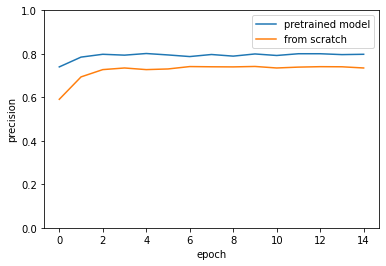
\includegraphics[scale=1.0]{figures/modeling.png}
\end{figure}

The pretrained data model have been trained from a massive data set. Using multi head attentions, the pretrained model could take advantage to learn different layers of knowledge about modeled language. Having been exposed to a more versatile set of locations of words inside sentence, it also has been able to capture more subtle attention for tokens inside input sentence.
All improvements achieving better results in quicker pace.

\section{Question 5}

Two languages modeling objective are proposed in \citep{bert2018}
\begin{itemize}
\item \textbf{Next Sentence Prediction (NSP)}. Our lab assignment objective is a close and limited version of such objective. We only learn short term dependency (next token) contrary to Bert objective which capture a longer dependancy and richer context. A full complete different sentence is to be learnt with a full set of potentially different tokens from source sentence
\item \textbf{Masked Language Model}. Noised version of sentences are built by artificially removing 15\% of tokens replaced by a special $unknown$ token. Through this sampling technique, Bert use a \textbf{bi directional} language modeling objective using simultaneously information for left to right and right to left traversal of input sentences. This is a major  change to lab assignement language modeling which only use left to right context through square mask.
\end{itemize}


\bibliographystyle{plain}
\bibliography{references} % citation records are in the references.bib document

\end{document}
